\documentclass[11pt]{article}
\usepackage[margin=2.2cm]{geometry}
\usepackage{amsmath,amssymb,amsthm}
\usepackage{booktabs,array,longtable,multirow}
\usepackage{graphicx}
\usepackage{float}
\usepackage[hidelinks]{hyperref}
\usepackage{enumitem}

\newcommand{\fillcell}{\rule[-0.75em]{0pt}{2.3em}}
\newcommand{\fillrow}{\rule[-0.4em]{0pt}{1.5em}}
\newcolumntype{C}[1]{>{\centering\arraybackslash}p{#1}}
\newcommand{\lgn}{\lfloor \log_2 n \rfloor}
\newcommand{\cha}{\text{`a'}}
\newcommand{\chb}{\text{`b'}}
\newcommand{\chc}{\text{`c'}}
\newtheorem{lemma}{Lemma}
\theoremstyle{remark}
\newtheorem*{claim}{Claim}

\title{CMPE 300: Analysis of Algorithms\\[0.3em] \large Project 1 Report --- Asymptotic \& Probabilistic Complexity Analysis}
\author{Yi\u{g}it Sarp Avc\i{}}
\date{November 2026}

\begin{document}
\maketitle

\section{Variant}

For our assigned variant ($key = (No_1 + No_2) \bmod 8 = 2$), the input symbol probabilities and loop division factor are:

\begin{center}
\begin{tabular}{|C{2.2cm}|C{2.2cm}|C{2.2cm}|C{2.2cm}|C{2.2cm}|}
\hline
\textbf{key} & $\boldsymbol{p_a}$ & $\boldsymbol{p_b}$ & $\boldsymbol{p_c}$ & $\boldsymbol{d}$ \\ \hline
\fillcell 2 & 1/3 & 1/3 & 1/3 & 2 \\ \hline
\end{tabular}
\end{center}

\noindent Throughout the report $n\ge 1$ is the input size, $\lg n=\log_2 n$, and
\[
  L(n) \;=\; \lgn + 1 .
\]

\section{Preliminaries}

\subsection{The while loop (lines 6--7)}

\begin{lemma}\label{lem:L}
For $n\ge 1$ and an integer $d\ge 2$ the while loop on lines 6--7 executes exactly
$\lfloor \log_d n\rfloor + 1$ times. For our variant ($d=2$) this is $L(n)=\lgn+1$.
Moreover $1\le L(n)\le n$.
\end{lemma}
\begin{proof}
Since $\lfloor\lfloor x\rfloor/d\rfloor=\lfloor x/d\rfloor$ for integer $d$, after $j$ iterations
$k=\lfloor n/d^j\rfloor$. The loop stops after iteration $j$ exactly when
$\lfloor n/d^j\rfloor=0$, i.e.\ $d^j>n$. The smallest such $j$ is
$\lfloor\log_d n\rfloor+1$ (the condition $k>0$ holds at the start because $n\ge1$).
Finally $2^{L-1}\le n$ and $L\le 2^{L-1}$ for every $L\ge1$, hence $L(n)\le n$.
\end{proof}

\subsection{Cost of one iteration of the outer loop}

Let $s_i$ denote the value of $s$ at the \emph{beginning} of iteration $i$ of the outer
loop ($s_0=0$). For a \chb\ the loop on line 9 runs for $q=0,\dots,s_i$, i.e.\
$s_i+1$ times, and the inner loop on line 11 runs $n$ times per $q$. For a \chc\ the loop on
line 15 runs for $t=i,\dots,n-1$, i.e.\ $n-i$ times. For loop increments (2) we count one
increment per iteration of the loops on lines 9 and 15 (the increment that moves the
loop variable to its next value; for \texttt{for q $\leftarrow$ 0 to s} there are $s+1$ of
them, the last one pushes $q$ to $s+1$ and terminates the loop).
The number of basic operations executed in iteration $i$ is therefore:

\begin{center}
\renewcommand{\arraystretch}{1.25}
\begin{tabular}{|c|c|c|c|c|}
\hline
$arr[i]$ & (1) comparisons & (2) loop increments & (3) assignments & (4) assignments \\ \hline
\cha & 1 & 0 & 1 & $L(n)$ \\ \hline
\chb & 2 & $s_i+1$ & $s_i+1$ & $(s_i+1)\,n$ \\ \hline
\chc & 2 & $n-i$ & 1 & $n-i$ \\ \hline
\end{tabular}
\end{center}

\noindent (For \chc\ the else branch has no comparison of its own; both comparisons on lines
3 and 8 are evaluated.) Note that the costs of \cha\ and \chc\ never depend on $s$; only
\chb\ depends on $s$. The variable $s$ obeys:
$s\leftarrow s+1$ on \cha, unchanged on \chb, $s\leftarrow 0$ on \chc. Hence
\begin{equation}\label{eq:s}
s_i = \text{number of \cha's in } arr[j..i-1], \quad j = 1 + (\text{index of the last \chc\ before } i)\ (\text{or } j=0),
\end{equation}
and in particular $0\le s_i\le i$ and $s_i\le$ (total number of \cha's in the input).

\begin{lemma}[monotonicity of $s$]\label{lem:mono}
Let $x$ be an input and $x'$ be obtained from $x$ by replacing one \chc\ at position $p$
by \cha\ or by \chb. Then $s'_i\ge s_i$ for every $i$.
\end{lemma}
\begin{proof}
For $i\le p$ the prefixes coincide, so $s'_i=s_i$. After position $p$:
$s_{p+1}=0\le s'_{p+1}$. From then on both strings are equal, so $s$ and $s'$ are updated by
the same rule ($+1$, unchanged, or reset to $0$); each rule preserves $s'\ge s$.
\end{proof}

\subsection{Random variables for the average case}

For the average case each $arr[i]$ is independently \cha, \chb, \chc\ with
probabilities $p_a=p_b=p_c=1/3$. We use
\begin{itemize}[nosep]
\item indicator random variables $X_i^{a},X_i^{b},X_i^{c}$, where $X_i^{x}=1$ iff $arr[i]=x$;
  $E[X_i^x]=p_x=1/3$;
\item the random variable $s_i$ (value of $s$ at the start of iteration $i$);
\item indicators $Y_{j,i}$ ($0\le j<i$): $Y_{j,i}=1$ iff $arr[j]=\cha$ and none of
  $arr[j+1],\dots,arr[i-1]$ is \chc.
\end{itemize}
By (\ref{eq:s}), an \cha\ at position $j<i$ is counted in $s_i$ exactly when no \chc\
occurs between it and $i$, so $s_i=\sum_{j=0}^{i-1} Y_{j,i}$. Using independence,
$E[Y_{j,i}]=p_a(1-p_c)^{i-1-j}$, therefore
\begin{equation}\label{eq:Es}
E[s_i]=\sum_{t=0}^{i-1}p_a(1-p_c)^t=\frac{p_a}{p_c}\bigl(1-(1-p_c)^i\bigr)
      = 1-\left(\tfrac{2}{3}\right)^i .
\end{equation}
Since $s_i$ depends only on $arr[0..i-1]$, it is \emph{independent} of $X_i^{b}$, so
$E[X_i^{b}(s_i+1)]=p_b\,(E[s_i]+1)$. Summing (\ref{eq:Es}) (a geometric series),
\begin{equation}\label{eq:sum}
\sum_{i=0}^{n-1}\bigl(E[s_i]+1\bigr) = 2n-\sum_{i=0}^{n-1}\left(\tfrac23\right)^i
 = 2n-3\Bigl(1-\left(\tfrac23\right)^n\Bigr) = 2n-3+3\left(\tfrac23\right)^n .
\end{equation}
Also $\sum_{i=0}^{n-1}(n-i)=\frac{n(n+1)}{2}$. Note how $s$ behaves in the average case:
it is \emph{not} $\approx$ (number of \cha's so far) $\approx i/3$, because every \chc\
(probability $1/3$) resets it; its expectation stays below $p_a/p_c=1$.

For every case the total count is $C=\sum_{i=0}^{n-1}\text{cost}_i$, and by linearity of
expectation $A(n)=\sum_i E[\text{cost}_i]$ where
$\text{cost}_i = X_i^a\,c_a + X_i^b\,c_b(s_i) + X_i^c\,c_c(i)$ with the costs of the table above.

% =====================================================================
\section{Theoretical Analysis}

\subsection{Case 1: comparisons (1)}

\paragraph{$B_1(n)$.} \emph{Best-case input:} $\cha^n$ (all \cha).
Every iteration executes the comparison on line 3, so every input of size $n$ executes at
least $n$ comparisons. For $\cha^n$ line 8 is never reached, so exactly $n$ comparisons are
made. No input can do fewer; moreover $\cha^n$ is the only best input, since any
\chb\ or \chc\ adds one comparison.
\[ B_1(n)=n\in\Theta(n). \]

\paragraph{$W_1(n)$.} \emph{Worst-case input:} $\chc^n$ (any input with no \cha, e.g.\ all
\chc\ or all \chb). Each iteration executes at most the two comparisons (lines 3 and 8),
so no input exceeds $2n$; an input without \cha\ executes both in every iteration.
\[ W_1(n)=2n\in\Theta(n). \]

\paragraph{$A_1(n)$.} Random variable: $C_1=\sum_{i=0}^{n-1} (X_i^a\cdot1+(X_i^b+X_i^c)\cdot2)$ (independent of $s$). By linearity of expectation,
\[ A_1(n)=E[C_1]=\sum_{i=0}^{n-1}\bigl(p_a+2(p_b+p_c)\bigr)=n\left(\tfrac13+\tfrac43\right)=\frac{5n}{3}\in\Theta(n). \]

\subsection{Case 2: loop increments (2)}

\paragraph{$B_2(n)$.} \emph{Best-case input:} $\cha^n$. Counts are non-negative, and for
$\cha^n$ neither loop (line 9, line 15) is entered, so the count is $0$. (It is the only
best input: any \chb\ costs $s_i+1\ge1$ and any \chc\ costs $n-i\ge1$.)
\[ B_2(n)=0\in\Theta(1). \]

\paragraph{$W_2(n)$.} \emph{Worst-case input:} $\chc^n$, count
$\sum_{i=0}^{n-1}(n-i)=n(n+1)/2$.

\emph{Proof that no input does more.} Take any input and split it into maximal
\emph{blocks} of consecutive non-\chc\ characters. Let a block occupy positions
$p,\dots,p+m-1$ ($m\ge1$) and contain $\alpha$ \cha's and $\beta$ \chb's ($\alpha+\beta=m$).
The block starts at the beginning or right after a \chc, so $s=0$ on entry and inside the
block $s_i\le\alpha$. The \cha's cost 0, so the block costs at most
$\beta(\alpha+1)=(m-\alpha)(\alpha+1)\le\left(\frac{m+1}{2}\right)^2$ (AM--GM).
Replace the whole block by \chc's. The new positions cost
$\sum_{i=p}^{p+m-1}(n-i)\ge\sum_{i=p}^{p+m-1}(p+m-i)=\frac{m(m+1)}{2}$, because
$p+m\le n$. Since $m\ge1$, $\frac{m(m+1)}2\ge\frac{(m+1)^2}{4}$, so the count does not
decrease. The costs of all other positions are unchanged: a \chc\ costs $n-i$ regardless
of its context, and every other block still starts with $s=0$ (it is still preceded by
the same \chc\ or by the start). Repeating for every block turns any input into $\chc^n$
without ever decreasing the count, so $\chc^n$ is a worst-case input:
\[ W_2(n)=\frac{n(n+1)}{2}\in\Theta(n^2). \]

\paragraph{$A_2(n)$.} Random variable: $C_2=\sum_{i=0}^{n-1}\bigl(X_i^b(s_i+1)+X_i^c(n-i)\bigr)$.
By linearity of expectation ($A_2(n)=E[C_2]$), the independence of $X_i^b$ and $s_i$, and (\ref{eq:sum}):
\[
A_2(n)=p_b\sum_{i=0}^{n-1}(E[s_i]+1)+p_c\sum_{i=0}^{n-1}(n-i)
=\frac{2n-3+3(2/3)^n}{3}+\frac{n(n+1)}{6}
=\frac{n^2+5n}{6}-1+\left(\tfrac23\right)^n\in\Theta(n^2).
\]

\subsection{Case 3: assignments (3)}

\paragraph{$B_3(n)$.} \emph{Best-case input:} $\cha^n$. Every iteration executes at least
one assignment of type (3) (\cha: line 4; \chb: line 10 runs $s_i+1\ge1$ times; \chc:
line 14), so every input executes at least $n$. $\cha^n$ executes exactly $n$.
(So do $\chb^n$, $\chc^n$ and every input in which every \chb\ has $s_i=0$; all of them are
best inputs, none does fewer.)
\[ B_3(n)=n\in\Theta(n). \]

\paragraph{$W_3(n)$.} \emph{Worst-case input:} $\cha^{\lfloor n/2\rfloor}\chb^{\lceil n/2\rceil}$.

\emph{Proof.} Step 1: replacing a \chc\ at position $p$ by \cha\ does not decrease the
count: position $p$ still costs 1, \cha/\chc\ costs elsewhere do not depend on $s$, and
by Lemma~\ref{lem:mono} every $s_i$ can only increase, so every \chb\ costs at least as
much. Hence there is a worst-case input over $\{\cha,\chb\}$.
Step 2: let such an input have $\alpha$ \cha's and $\beta=n-\alpha$ \chb's. Each
\chb\ costs $s_i+1\le\alpha+1$, so the count is at most $\alpha+\beta(\alpha+1)$, with
equality iff all \cha's precede all \chb's ($\cha^\alpha\chb^\beta$).
Step 3: $f(\alpha)=\alpha+(n-\alpha)(\alpha+1)=-\alpha^2+n\alpha+n$ is a concave parabola
with vertex $\alpha=n/2$, so over integers it is maximised at $\alpha=\lfloor n/2\rfloor$
(also at $\lceil n/2\rceil$). Since $\lfloor n/2\rfloor+\lceil n/2\rceil=n$ and
$\lfloor n/2\rfloor\lceil n/2\rceil=\lfloor n^2/4\rfloor$, we obtain
\[
W_3(n)=\lfloor n/2\rfloor+\lceil n/2\rceil\bigl(\lfloor n/2\rfloor+1\bigr)
=\left\lfloor\frac{n^2}{4}\right\rfloor+n\in\Theta(n^2).
\]

\paragraph{$A_3(n)$.} Random variable: $C_3=\sum_{i=0}^{n-1}\bigl(X_i^a+X_i^b(s_i+1)+X_i^c\bigr)$.
\[
A_3(n)=E[C_3]=(p_a+p_c)\,n+p_b\sum_{i=0}^{n-1}(E[s_i]+1)=\frac{2n}{3}+\frac{2n-3+3(2/3)^n}{3}
=\frac{4n}{3}-1+\left(\tfrac23\right)^n\in\Theta(n).
\]

\subsection{Case 4: assignments (4)}

\paragraph{$B_4(n)$.} \emph{Best-case input:} $\cha^{\,n-L+1}\chc^{\,L-1}$ with
$L=L(n)=\lgn+1$ (i.e.\ \cha\ at positions $0,\dots,n-L$ and \chc\ at the last $L-1$
positions).

\emph{Proof.} By the table, position $i$ costs $L$ if it is \cha, $(s_i+1)n\ge n$ if it is
\chb, and $n-i$ if it is \chc. By Lemma~\ref{lem:L}, $L\le n$, so whatever the input,
position $i$ costs at least $\min(L,\,n-i)$ and every input costs at least
$\sum_{i=0}^{n-1}\min(L,n-i)$. Because \cha\ and \chc\ costs do not depend on $s$, putting
\chc\ exactly where $n-i<L$ (i.e.\ $i\ge n-L+1$) and \cha\ elsewhere achieves this bound.
Positions $0..n-L$ cost $L$ each and the last $L-1$ positions cost $L-1,\dots,1$:
\[
B_4(n)=(n-L+1)L+\frac{L(L-1)}{2}=\frac{L(2n-L+1)}{2}
=\frac{(\lgn+1)(2n-\lgn)}{2}\in\Theta(n\log n),
\]
since $n+1\le 2n-L+1\le 2n$.

\paragraph{$W_4(n)$.} \emph{Worst-case input:}
$\cha^{\lfloor n/2\rfloor}\chb^{\lceil n/2\rceil}$.

\emph{Proof.} Step 1: replacing a \chc\ at position $p$ by \chb\ never decreases the count:
position $p$ goes from $n-p\le n$ to $(s_p+1)n\ge n$; by Lemma~\ref{lem:mono} all later
$s_i$ can only grow, so every later \chb\ costs at least as much, and \cha/\chc\ costs are
unchanged. Hence a worst-case input exists over $\{\cha,\chb\}$.
Step 2: with $\alpha$ \cha's and $\beta=n-\alpha$ \chb's, each \chb\ costs
$(s_i+1)n\le(\alpha+1)n$, so the count is at most $g(\alpha)=\alpha L+n(n-\alpha)(\alpha+1)$,
with equality iff the input is $\cha^\alpha\chb^\beta$.
Step 3: $g(\alpha)=-n\alpha^2+(n^2-n+L)\alpha+n^2$ has forward difference
$g(\alpha+1)-g(\alpha)=L+n(n-2\alpha-2)$ and vertex
$\alpha^*=\frac{n-1}{2}+\frac{L}{2n}$, where $0<\frac{L}{2n}\le\frac12$ (Lemma~\ref{lem:L}).
For integer $\alpha<\lfloor n/2\rfloor$ we have $2\alpha\le n-2$ and thus $n-2\alpha-2\ge 0$, so $g(\alpha+1)-g(\alpha)\ge L>0$;
for integer $\alpha\ge\lfloor n/2\rfloor$ we have $2\alpha\ge n-1$ and thus $n-2\alpha-2\le -1$, so $g(\alpha+1)-g(\alpha)\le L-n\le 0$.
Thus $g(\alpha)$ is maximised over integers at $\alpha=\lfloor n/2\rfloor$, giving
\[
W_4(n)=\lfloor n/2\rfloor(\lgn+1)+n\lceil n/2\rceil\bigl(\lfloor n/2\rfloor+1\bigr)\in\Theta(n^3)
\]
(the second term is $\approx n^3/4$).

\paragraph{$A_4(n)$.} Random variable: $C_4=\sum_{i=0}^{n-1}\bigl(X_i^aL+X_i^b(s_i+1)n+X_i^c(n-i)\bigr)$.
\begin{align*}
A_4(n)=E[C_4]&=p_a nL+p_b\,n\sum_{i=0}^{n-1}(E[s_i]+1)+p_c\sum_{i=0}^{n-1}(n-i)
=\frac{nL}{3}+\frac{n\bigl(2n-3+3(2/3)^n\bigr)}{3}+\frac{n(n+1)}{6}\\
&=\frac{5n^2-5n}{6}+\frac{n(\lgn+1)}{3}+n\left(\tfrac23\right)^n\in\Theta(n^2).
\end{align*}

\subsection*{Checking the formulas}
Besides the counter runs of Section~\ref{sec:verify}, we enumerated \emph{all} $3^n$
inputs for every $n\le 9$ with the counting implementation: the minimum and maximum
counts equal $B_k(n)$ and $W_k(n)$ for all four cases, they are attained by the inputs given
above, and the exact (probability-weighted) mean equals $A_k(n)$.

\subsection*{Table 1: Theoretical Analysis Results}

\begin{longtable}{|C{2.3cm}|C{1.5cm}|p{7.2cm}|C{3.0cm}|}
\hline
\textbf{Basic operation} & \textbf{Case} & \centering\arraybackslash\textbf{Exact count (closed form)} & \textbf{Asymptotic} \\ \hline
\endhead
\hline
\endfoot
\multirow{3}{*}{\parbox{2.3cm}{\centering (1)\\comparisons}}
 & $B_1(n)$ & \fillcell $n$ & $\Theta(n)$ \\ \cline{2-4}
 & $W_1(n)$ & \fillcell $2n$ & $\Theta(n)$ \\ \cline{2-4}
 & $A_1(n)$ & \fillcell $\dfrac{5n}{3}$ & $\Theta(n)$ \\ \hline
\multirow{3}{*}{\parbox{2.3cm}{\centering (2)\\loop increments}}
 & $B_2(n)$ & \fillcell $0$ & $\Theta(1)$ \\ \cline{2-4}
 & $W_2(n)$ & \fillcell $\dfrac{n(n+1)}{2}$ & $\Theta(n^2)$ \\ \cline{2-4}
 & $A_2(n)$ & \fillcell $\dfrac{n^2+5n}{6}-1+\left(\frac23\right)^n$ & $\Theta(n^2)$ \\ \hline
\multirow{3}{*}{\parbox{2.3cm}{\centering (3)\\assignments}}
 & $B_3(n)$ & \fillcell $n$ & $\Theta(n)$ \\ \cline{2-4}
 & $W_3(n)$ & \fillcell $\left\lfloor\dfrac{n^2}{4}\right\rfloor+n$ & $\Theta(n^2)$ \\ \cline{2-4}
 & $A_3(n)$ & \fillcell $\dfrac{4n}{3}-1+\left(\frac23\right)^n$ & $\Theta(n)$ \\ \hline
\multirow{3}{*}{\parbox{2.3cm}{\centering (4)\\assignments}}
 & $B_4(n)$ & \fillcell $\dfrac{(\lgn+1)(2n-\lgn)}{2}$ & $\Theta(n\log n)$ \\ \cline{2-4}
 & $W_4(n)$ & \fillcell $\lfloor\frac n2\rfloor(\lgn+1)+n\lceil\frac n2\rceil(\lfloor\frac n2\rfloor+1)$ & $\Theta(n^3)$ \\ \cline{2-4}
 & $A_4(n)$ & \fillcell $\dfrac{5n^2-5n}{6}+\dfrac{n(\lgn+1)}{3}+n\left(\frac23\right)^n$ & $\Theta(n^2)$ \\ \hline
\end{longtable}

% =====================================================================
\section{Real Execution}

\subsection{The ``correct'' basic operation}

The operation that characterises the algorithm is set \textbf{(4)}: the assignments on
lines 7, 12 and 16. They are the statements in the innermost loop of \emph{every} branch
(line 12 is inside two nested loops). In every iteration of the outer loop at least one
(4)-assignment is executed (\cha: $L\ge1$, \chb: $(s_i+1)n\ge1$, \chc: $n-i\ge1$), and all
other work of an iteration is $O(1)$ plus $O(1)$ per (4)-assignment (every loop test,
increment, comparison and the other assignments are charged to one execution of a
line-7/12/16 assignment or to the $O(1)$ overhead of the iteration). Hence the running time
is $\Theta(C_4)$ for every input, where $C_4$ is the number of (4)-assignments.

\emph{Consistency of the four analyses.} The other three sets are not consistent with the
real cost of the algorithm:
\begin{itemize}[nosep]
\item (1) only sees one or two comparisons per iteration and says the algorithm is
  always linear; it does not see any inner loop.
\item (2) ignores the while loop and the $r$-loop. For $\cha^n$ it gives 0 although
  $\Theta(n\log n)$ work is done, and its worst input $\chc^n$ is \emph{not} the worst input of the
  algorithm ($\chc^n$ costs only $n(n+1)/2$ assignments (4), whereas
  $\cha^{\lfloor n/2\rfloor}\chb^{\lceil n/2\rceil}$ costs $\Theta(n^3)$).
\item (3) counts the $q$-loop but not the $r$-loop nested in it, so it misses a factor $n$
  ($W_3\in\Theta(n^2)$ instead of $\Theta(n^3)$, $A_3\in\Theta(n)$ instead of $\Theta(n^2)$), and its best case misses the $\log n$ factor of the while loop.
\end{itemize}
Only set (4) gives the true orders $\Theta(n\log n)$, $\Theta(n^3)$, $\Theta(n^2)$. The
best-, worst- and average-case inputs used below are therefore those of case (4):
best $\cha^{\,n-L+1}\chc^{\,L-1}$, worst $\cha^{\lfloor n/2\rfloor}\chb^{\lceil n/2\rceil}$,
average: random arrays with $p_a=p_b=p_c=1/3$, 10 runs per size, averaged.

\subsection*{Table 2: Real Execution Times}

Basic operation identified as the ``correct'' one: \underline{(4) assignments, lines 7, 12, 16}\\[0.4em]
Programming language / machine: \underline{Python 3.12.9 (CPython)} /\\
\underline{Intel Core i7-13700H laptop, 32 GB RAM, Windows 11}

\begin{center}
\begin{tabular}{|C{1.6cm}|C{3.4cm}|C{3.4cm}|C{3.8cm}|}
\hline
$n$ & \textbf{Best (s)} & \textbf{Worst (s)} & \textbf{Average (s)} \\ \hline
1 & \fillrow 0.000001500 & 0.000001100 & 0.000000630 \\ \hline
5 & \fillrow 0.000002700 & 0.000003200 & 0.000001720 \\ \hline
10 & \fillrow 0.000002200 & 0.000013200 & 0.000003650 \\ \hline
20 & \fillrow 0.000003700 & 0.000075600 & 0.000015040 \\ \hline
40 & \fillrow 0.000007900 & 0.000500000 & 0.000044940 \\ \hline
50 & \fillrow 0.000009500 & 0.001156000 & 0.000063670 \\ \hline
60 & \fillrow 0.000011300 & 0.001719200 & 0.000099850 \\ \hline
80 & \fillrow 0.000016200 & 0.003732400 & 0.000151920 \\ \hline
100 & \fillrow 0.000020200 & 0.006754300 & 0.000261490 \\ \hline
150 & \fillrow 0.000032400 & 0.023097300 & 0.000542950 \\ \hline
200 & \fillrow 0.000043800 & 0.054622700 & 0.000909290 \\ \hline
250 & \fillrow 0.000054700 & 0.109360300 & 0.001489160 \\ \hline
300 & \fillrow 0.000075300 & 0.204555200 & 0.002306830 \\ \hline
350 & \fillrow 0.000085400 & 0.347920700 & 0.003400350 \\ \hline
400 & \fillrow 0.000099600 & 0.536697400 & 0.004937900 \\ \hline
\end{tabular}
\end{center}

Times were measured with \texttt{time.perf\_counter()} around a call of the counter-free
implementation only (input generation is not timed). The individual times of the 10
average-case runs are printed by the program right below each average-case line.
For $n\le5$ the times are a few microseconds and are dominated by function-call overhead and
timer resolution, which is why e.g.\ the best time at $n=1$ is not smaller than the worst time.

% =====================================================================
\section{Exact Count Verification}\label{sec:verify}

The program has a second implementation, \texttt{algorithm\_counted}, with one counter per
set (1)--(4); it is never used for timing. The command \texttt{--verify} runs it on the best
and worst inputs of each case (for cases (1) and (2) the best input is $\cha^n$ and the worst
$\chc^n$; for case (3) best $\cha^n$, worst $\cha^{\lfloor n/2\rfloor}\chb^{\lceil n/2\rceil}$;
for case (4) best $\cha^{n-L+1}\chc^{L-1}$, worst $\cha^{\lfloor n/2\rfloor}\chb^{\lceil n/2\rceil}$),
and on $N=2000$ random inputs per $n$ (seed 300).

\subsection*{Table 3: Exact Count Verification (Best and Worst Case)}

\begin{longtable}{|C{2.3cm}|C{1.2cm}|C{2.6cm}|C{2.6cm}|C{2.6cm}|C{2.6cm}|}
\hline
\textbf{Basic operation} & $\boldsymbol{n}$ & \textbf{Counted best} & \textbf{Formula $B(n)$} & \textbf{Counted worst} & \textbf{Formula $W(n)$} \\ \hline
\endhead
\hline
\endfoot
\multirow{6}{*}{\parbox{2.3cm}{\centering (1)\\comparisons}} & 1 & \fillrow 1 & 1 & 2 & 2 \\ \cline{2-6}
 & 5 & \fillrow 5 & 5 & 10 & 10 \\ \cline{2-6}
 & 10 & \fillrow 10 & 10 & 20 & 20 \\ \cline{2-6}
 & 20 & \fillrow 20 & 20 & 40 & 40 \\ \cline{2-6}
 & 40 & \fillrow 40 & 40 & 80 & 80 \\ \cline{2-6}
 & 100 & \fillrow 100 & 100 & 200 & 200 \\ \hline
\multirow{6}{*}{\parbox{2.3cm}{\centering (2)\\loop increments}} & 1 & \fillrow 0 & 0 & 1 & 1 \\ \cline{2-6}
 & 5 & \fillrow 0 & 0 & 15 & 15 \\ \cline{2-6}
 & 10 & \fillrow 0 & 0 & 55 & 55 \\ \cline{2-6}
 & 20 & \fillrow 0 & 0 & 210 & 210 \\ \cline{2-6}
 & 40 & \fillrow 0 & 0 & 820 & 820 \\ \cline{2-6}
 & 100 & \fillrow 0 & 0 & 5050 & 5050 \\ \hline
\multirow{6}{*}{\parbox{2.3cm}{\centering (3)\\assignments}} & 1 & \fillrow 1 & 1 & 1 & 1 \\ \cline{2-6}
 & 5 & \fillrow 5 & 5 & 11 & 11 \\ \cline{2-6}
 & 10 & \fillrow 10 & 10 & 35 & 35 \\ \cline{2-6}
 & 20 & \fillrow 20 & 20 & 120 & 120 \\ \cline{2-6}
 & 40 & \fillrow 40 & 40 & 440 & 440 \\ \cline{2-6}
 & 100 & \fillrow 100 & 100 & 2600 & 2600 \\ \hline
\multirow{6}{*}{\parbox{2.3cm}{\centering (4)\\assignments}} & 1 & \fillrow 1 & 1 & 1 & 1 \\ \cline{2-6}
 & 5 & \fillrow 12 & 12 & 51 & 51 \\ \cline{2-6}
 & 10 & \fillrow 34 & 34 & 320 & 320 \\ \cline{2-6}
 & 20 & \fillrow 90 & 90 & 2250 & 2250 \\ \cline{2-6}
 & 40 & \fillrow 225 & 225 & 16920 & 16920 \\ \cline{2-6}
 & 100 & \fillrow 679 & 679 & 255350 & 255350 \\ \hline
\end{longtable}

All 48 counted values are equal to the values of the formulas, as expected for exact analyses.

\clearpage
\subsection*{Table 4: Exact Count Verification (Average Case)}

\noindent Number of random inputs used for each $n$ ($N\ge 1000$): \underline{2000}

\begin{center}
\begin{longtable}{|C{2.3cm}|C{1.2cm}|C{3.4cm}|C{3.0cm}|C{2.8cm}|}
\hline
\textbf{Basic operation} & $\boldsymbol{n}$ & \textbf{Mean of counted values} & \textbf{Formula $A(n)$} & \textbf{Difference} \\ \hline
\endhead
\hline
\endfoot
\multirow{3}{*}{\parbox{2.3cm}{\centering (1)\\comparisons}} & 10 & \fillrow 16.677 & 16.667 & {\footnotesize $+0.011$ ($+0.07\%$)} \\ \cline{2-5}
 & 40 & \fillrow 66.651 & 66.667 & {\footnotesize $-0.016$ ($-0.02\%$)} \\ \cline{2-5}
 & 100 & \fillrow 166.703 & 166.667 & {\footnotesize $+0.037$ ($+0.02\%$)} \\ \hline
\multirow{3}{*}{\parbox{2.3cm}{\centering (2)\\loop increments}} & 10 & \fillrow 24.008 & 24.017 & {\footnotesize $-0.009$ ($-0.04\%$)} \\ \cline{2-5}
 & 40 & \fillrow 298.240 & 299.000 & {\footnotesize $-0.760$ ($-0.25\%$)} \\ \cline{2-5}
 & 100 & \fillrow 1750.037 & 1749.000 & {\footnotesize $+1.037$ ($+0.06\%$)} \\ \hline
\multirow{3}{*}{\parbox{2.3cm}{\centering (3)\\assignments}} & 10 & \fillrow 12.241 & 12.351 & {\footnotesize $-0.110$ ($-0.89\%$)} \\ \cline{2-5}
 & 40 & \fillrow 52.523 & 52.333 & {\footnotesize $+0.189$ ($+0.36\%$)} \\ \cline{2-5}
 & 100 & \fillrow 132.048 & 132.333 & {\footnotesize $-0.285$ ($-0.22\%$)} \\ \hline
\multirow{3}{*}{\parbox{2.3cm}{\centering (4)\\assignments}} & 10 & \fillrow 87.068 & 88.507 & {\footnotesize $-1.439$ ($-1.63\%$)} \\ \cline{2-5}
 & 40 & \fillrow 1388.025 & 1380.000 & {\footnotesize $+8.025$ ($+0.58\%$)} \\ \cline{2-5}
 & 100 & \fillrow 8463.554 & 8483.333 & {\footnotesize $-19.779$ ($-0.23\%$)} \\ \hline
\end{longtable}
\end{center}

\paragraph{Comment on the differences.} $A(n)$ is an expectation, whereas the table shows
the mean of a finite sample of 2000 random inputs, so small differences are expected; all
are below $2\%$ and change sign randomly, i.e.\ they are sampling noise, not a systematic
error. For case (1) the per-input count is $n+(\#\chb+\#\chc)$, which has small variance, so
the error is tiny ($<0.1\%$). Cases (2)--(4) depend on $s$ and on the positions of the
\chc's, so their counts vary much more from input to input (for case (4) a single \chb\
after many \cha's costs $\Theta(n\cdot s)$); this gives the larger absolute differences,
e.g.\ $-1.6\%$ for case (4) at $n=10$. The standard error decreases as $1/\sqrt N$, and the
exhaustive enumeration for $n\le9$ (Section 3) confirms that the formulas are the exact
expectations.

% =====================================================================
\section{Comparison of Theoretical Analysis and Real Behavior}

Figure~\ref{fig:c4} compares the theoretical operation counts of basic-operation set \textbf{(4)}
(identified as the correct basic operation in Section~4) against the measured execution times
from Table~2 across all 15 input sizes $n\in\{1,5,10,\dots,400\}$ for the best, worst, and
average cases. In each panel, the blue curve (left axis) displays the exact theoretical count
($B_4(n)$, $W_4(n)$, or $A_4(n)$), while the orange markers (right axis) show the measured
execution time in seconds. Figure~\ref{fig:times} shows all 45 timing records on linear and
log--log axes, and Figure~\ref{fig:ratio} displays the empirical time-per-operation ratio
($\text{time}/C_4$) alongside the three theoretical curves on a logarithmic scale.

\begin{figure}[H]
\centering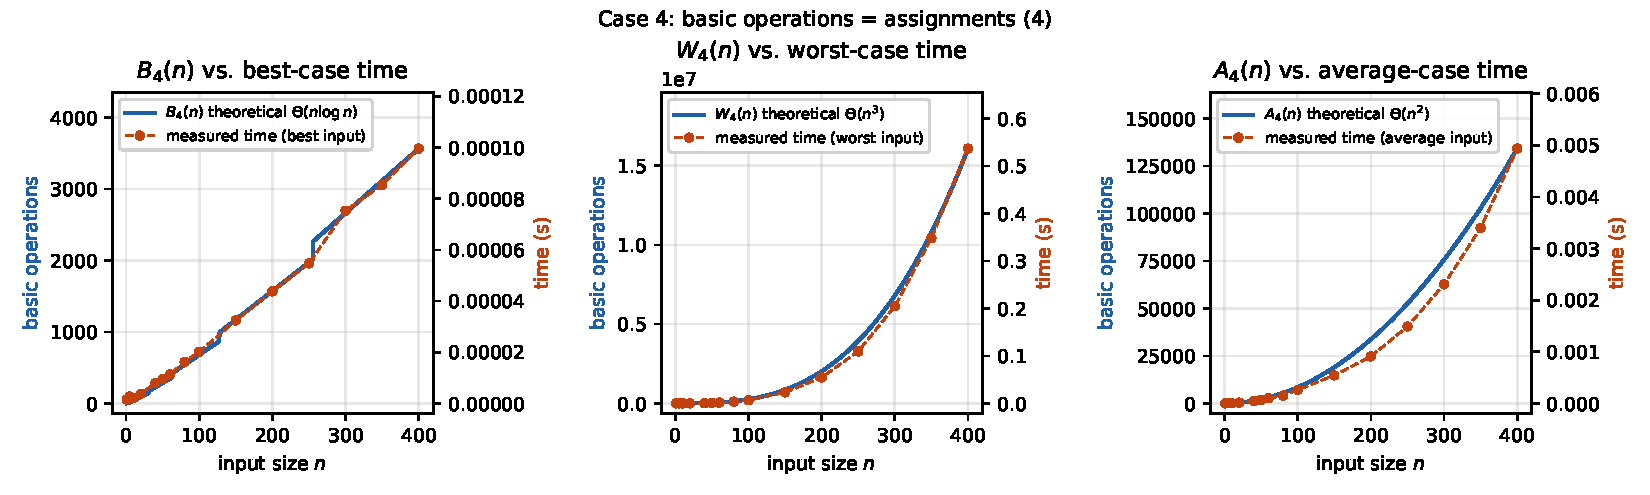
\includegraphics[width=\textwidth]{figures/case4.pdf}
\caption{Case (4), assignments on lines 7, 12, 16: theoretical counts $B_4(n)$, $W_4(n)$, and $A_4(n)$ vs.\ measured execution times.}\label{fig:c4}
\end{figure}

\begin{figure}[H]
\centering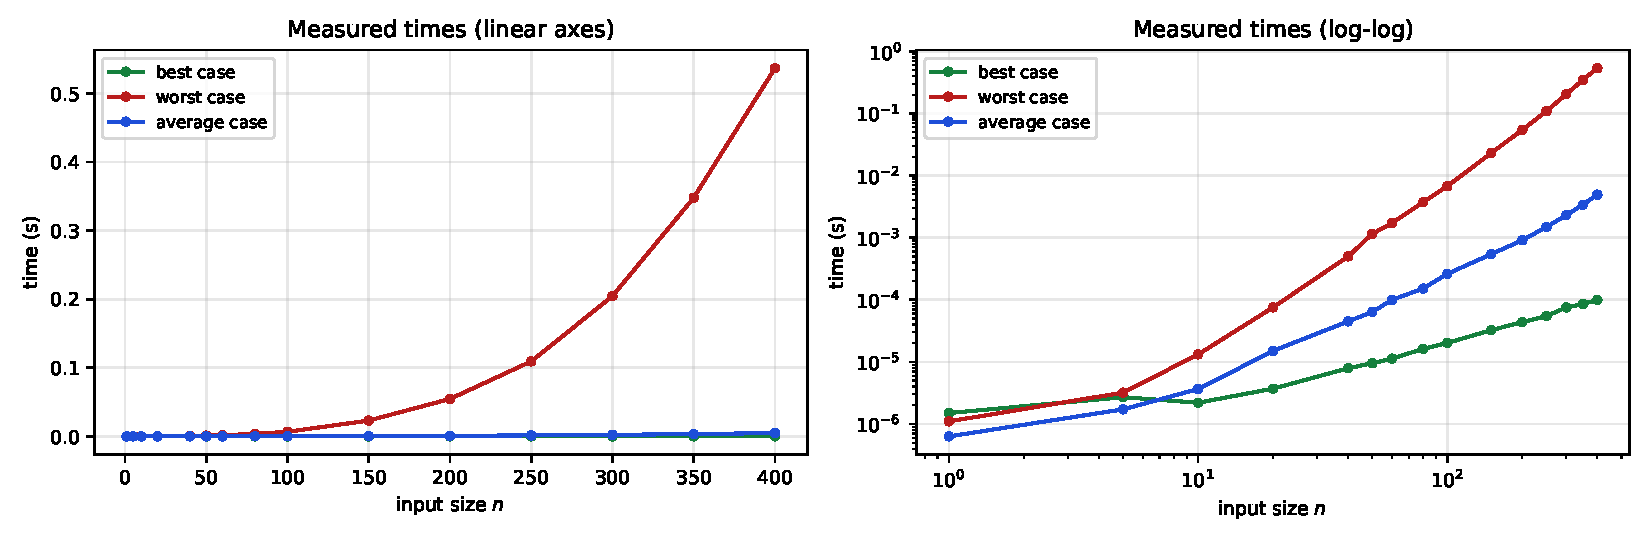
\includegraphics[width=\textwidth]{figures/times.pdf}
\caption{All 45 measured execution times on linear axes (left) and log--log axes (right). On the log--log plot, the empirical slopes for large $n$ are approximately $1$ (best case), $3$ (worst case), and $2$ (average case).}\label{fig:times}
\end{figure}

\begin{figure}[H]
\centering
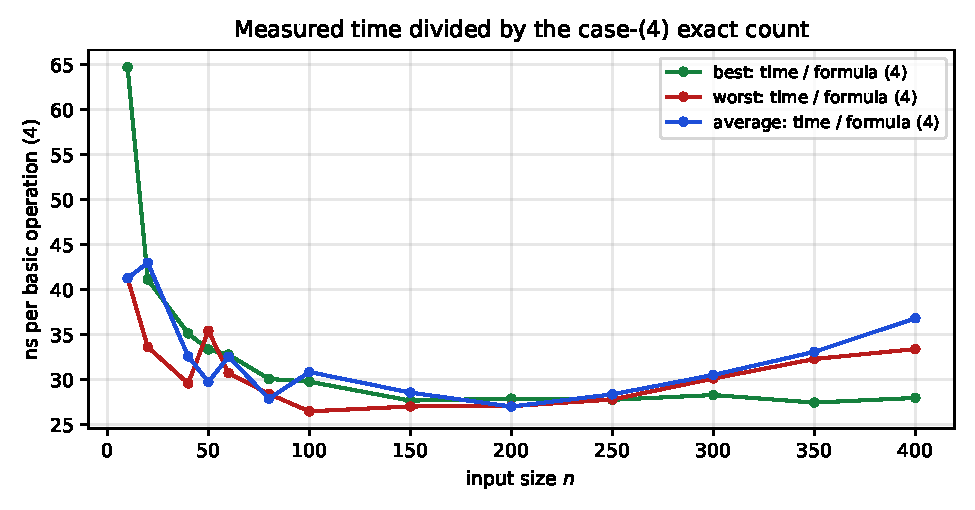
\includegraphics[width=0.49\textwidth]{figures/ratio.pdf}\hfill
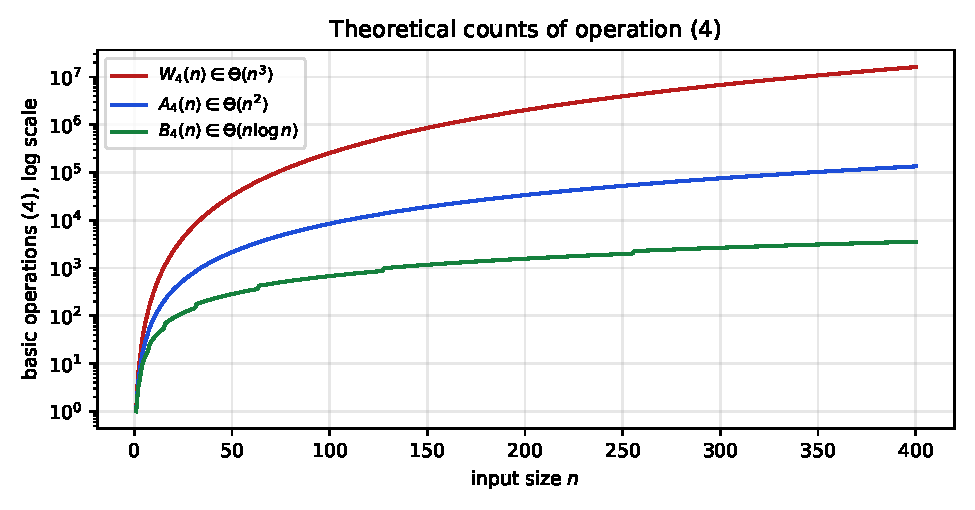
\includegraphics[width=0.49\textwidth]{figures/theory4.pdf}
\caption{Left: measured time divided by the exact count of operation (4) for $n\ge10$ (ns per operation).
Right: theoretical counts $B_4(n)$, $W_4(n)$, and $A_4(n)$ on a logarithmic scale.}\label{fig:ratio}
\end{figure}

\clearpage
\subsection*{Comments on the comparisons for basic-operation set (4)}

\begin{enumerate}[label=\textbf{(\arabic*)},nosep]
\item \textbf{Best case: $B_4(n)=\frac{(\lgn+1)(2n-\lgn)}{2}\in\Theta(n\log n)$.}
  The theoretical $B_4(n)$ curve matches the measured best-case execution times closely across the entire range of $n$ (Figure~\ref{fig:c4}, left panel). The slight discrete slope changes in $B_4(n)$ occur where $\lgn$ increments at powers of $2$ (such as $n=128$ and $n=256$), and the empirical timing curve follows the same quasi-linear trajectory. For $n\ge50$, the ratio $\text{time}/B_4(n)$ remains flat between $28$ and $34$\,ns per operation (Figure~\ref{fig:ratio}, left), confirming that actual best-case running time is directly proportional to $B_4(n)$. For very small sizes ($n\le10$), fixed interpreter and function-call overhead ($1$--$3\,\mu\text{s}$) dominates the sub-microsecond loop cost, explaining why the ratio starts higher before converging to a constant.

\item \textbf{Worst case: $W_4(n)=\lfloor\frac n2\rfloor(\lgn+1)+n\lceil\frac n2\rceil(\lfloor\frac n2\rfloor+1)\in\Theta(n^3)$.}
  The cubic theoretical curve $W_4(n)$ and the measured worst-case times overlap almost identically (Figure~\ref{fig:c4}, middle panel). When $n$ quadruples from $100$ to $400$, $W_4(n)$ increases by a factor of $16{,}081{,}800 / 255{,}350 \approx 63.0 \approx 4^3$, and the measured worst-case time increases from $0.00675$\,s to $0.53670$\,s (a factor of $\approx 79.5$). Consistently, the ratio $\text{time}/W_4(n)$ stays nearly constant between $26$ and $36$\,ns per operation for $n\ge50$, and the log--log plot (Figure~\ref{fig:times}, right) exhibits a clear asymptotic slope of $3$.

\item \textbf{Average case: $A_4(n)=\frac{5n^2-5n}{6}+\frac{n(\lgn+1)}3+n(2/3)^n\in\Theta(n^2)$.}
  The quadratic theoretical curve $A_4(n)$ accurately tracks the 10-run mean execution times (Figure~\ref{fig:c4}, right panel). When $n$ doubles from $100$ to $200$, $A_4(n)$ grows by a factor of $33{,}700.0 / 8{,}483.3 \approx 3.97 \approx 2^2$, and the measured average time grows from $0.00026$\,s to $0.00091$\,s (and to $0.00494$\,s at $n=400$). For $n\ge50$, the ratio $\text{time}/A_4(n)$ stays within $27$--$37$\,ns per operation (matching the per-operation cost observed in the best and worst cases), and the log--log plot shows a slope of $2$. The minor local fluctuations around the smooth curve are caused by finite-sample variance across the 10 random inputs per size and OS scheduling jitter.
\end{enumerate}

\vspace{-0.6em}
\paragraph{Average case vs.\ worst case.} The worst case is $\Theta(n^3)$ but the average case is
only $\Theta(n^2)$; at $n=400$ the worst time (0.537\,s) is about 109 times the average time
(0.0049\,s), close to $W_4(400)/A_4(400)\approx 1.6\cdot10^7/1.34\cdot10^5\approx120$.
The reason is visible in the pseudocode. The only cubic term comes from lines 9--12: a \chb\
costs $(s+1)\cdot n$ assignments, and $s$ counts the \cha's seen since the last \chc. In the
worst case all $\lfloor n/2\rfloor$ \cha's come first and are never reset, so each of the
$\approx n/2$ \chb's costs $\approx n^2/2$, giving $\approx n^3/4$. In a random input, however,
every element is a \chc\ with probability $1/3$ and line 14 resets $s$ to 0, so $s$ never
accumulates: $E[s_i]=1-(2/3)^i<1$ (Section 2.3). Thus an average \chb\ costs fewer than $2n$
assignments, the $n/3$ expected \chb's contribute $\Theta(n^2)$, the \chc's contribute
$\frac13\cdot\frac{n(n+1)}2=\Theta(n^2)$ through line 16, and the \cha's only
$\Theta(n\log n)$ through line 7. Hence $A_4(n)\in\Theta(n^2)$.

\vspace{-0.6em}
% =====================================================================
\section{Code}

The implementation is a self-contained Python 3 module (\texttt{complexity\_analyzer.py}, standard library only). It evaluates Variant 2 and prints \texttt{Variant: 2 (p\_a=1/3, p\_b=1/3, p\_c=1/3, d=2)} followed by the requested mode output:
\begin{itemize}[nosep]
\item \texttt{python3 complexity\_analyzer.py} --- prints the 45 timing lines of the form
  \texttt{Case: <case> Size: <size> Elapsed Time (s): <time>} (best, worst, average; for every
  average line the 10 individual run times are printed below it).
\item \texttt{python3 complexity\_analyzer.py --count aabcbba} --- prints the variant line
  and \texttt{Count(1): 11 Count(2): 9 Count(3): 9 Count(4): 48}.
\item \texttt{python3 complexity\_analyzer.py --verify} --- prints the data of Tables 3 and 4.
\end{itemize}
\texttt{algorithm} (no counters) is used for timing; \texttt{algorithm\_counted} (four
counters) is used by the count and verify modes.

\end{document}
